\chapter[Introduction]{Introduction} \label{ch:intro}

% I have seen the dark universe yawning, Where the black planets roll without
% aim; Where they roll in their horror unheeded, without knowledge or lustre or
% name. - Lovecraft

% All you really need to know for the moment is that the universe is a lot more
% complicated than you might think, even if you start from a position of
% thinking it's pretty damn complicated in the first place. - Douglas Adams

% In the beginning the Universe was created. This has made a lot of people very
% angry and been widely regarded as a bad move. - Douglas Adams

\vspace{-16pt} \begin{chapquote}{Douglas Adams} \singlespacing There is a theory
which states that if ever anyone discovers exactly what the Universe is for and
why it is here, it will instantly disappear and be replaced by something even
more bizarre and inexplicable. There is another theory which states that this
has already happened. \end{chapquote} \vspace{-8pt}
\noindent\makebox[\linewidth]{\rule{0.5\textwidth}{0.5pt}} \vspace{1pt}

To many, the Milky Way represents the faint, fuzzy band of light that arcs
across a dark, moonless sky.\footnote{But not to anyone who lives in New York
City, where the majority of the research presented in this \article\ was
conducted.} Long suspected to be a collection of unresolved stars (as early as
the 1200s), Galileo Galilei confirmed this idea using the first astronomical
telescopes in the 1600s. By 1755, Immanuel Kant speculated that the Milky Way
may appear thin across the sky because we are viewing a large disk of stars from
within, like a scaled-up version of the solar system with many more bodies
(stars). Between then and the early 1900s, hundreds of ``spiral nebulae'' were
discovered that were initially believed to be either star-forming regions within
the Milky Way or external ``island universes.'' It took Edwin Hubble's distance
measurements to the nearby galaxies M31 and M33---enabled by the concerted
efforts of many astronomers---to clearly place them outside of the Milky Way and
thus place our own Galaxy in the context of the universe of other galaxies.

Since the mid-1900s, through decades of research studying the structure of stars
and gas at ever-increasing distances, we now know a great deal more about the
Milky Way. Its scales are vast: the Galaxy hosts at least 100 billion stars over
a distance of about 3 billion billion kilometers and took about 13 billion years
to form to present day. But even more surprising than what we have observed is
what we haven't: from the motion of gas in the outer Galaxy, the velocities of
stars in external galaxies, and the gravitational lensing of distant galaxies,
we now know that---by mass---the dominant substance in the universe is unseen,
\emph{dark matter}.

Constraints on cosmological parameters from many independent sources---e.g., the
cosmic microwave background \citep{planck15}, Type Ia supernova distances
\citep{riess98, perlmutter99}, and baryon acoustic oscillations
\citep{eisenstein05}---have found that the energy density of the universe is
dominated by dark energy ($\approx$73\%) and dark matter ($\approx$23\%).
Ordinary baryonic matter constitutes a meager 4\% of this energy density and at
present is the only observable tracer of the vastly more numerous dark matter
\citep[though the search for the dark matter particle is
underway;][]{aprile11,luxdm12}. Dark matter dominates the mass of galaxies on
large scales and choreographs their interactions. Therefore, the basis for
expanding our understanding of the universe will come through characterization
and detection of dark matter. The goal of the work presented in this \article\
is to develop methods to further our understanding of the global potential of
the Milky Way in order to connect the Galaxy to cosmological predictions and---
for the first time---precisely measure the structure of dark matter around a
galaxy.

% Some of the most pertinent questions of our time are: What is the nature of
% dark matter? How does the milky way fit in to cosmology / galaxy formation?]

\todo{fill in this paragraph}
In what follows, Galactocentric quantities are generally shown with no
subscript, e.g., spherical radius $r$, cylindrical radius $R$. Heliocentric
quantities use the [...] symbol in subscript---e.g., radial distance from the
sun $r_\odot$. Capital, italicized galaxy components such as \mwdisk, \mwbulge,
and \mwhalo\ refer to components of the Milky Way, whereas in lower-case these
words refer to the components in general.

\section{The Milky Way} \label{sec:milkyway}

In its global properties, the Milky Way is a fairly typical disk galaxy. It is,
however, the one galaxy for which it is presently possible to measure detailed
chemical abundances and full-space positions and velocities for large samples of
individual stars (see Section~\ref{sec:mw-surveys} for an overview of surveys
that are measuring or will measure these chemo-dynamical quantities for stars in
the outer Galaxy). This is of great interest to modeling the formation and
evolution of the Galaxy: while a given star is born with a unique, frozen-in
chemical ``tag'' apparent in its surface chemical abundances, the kinematics of
the star will evolve from its birth location (in phase-space) due to dynamical
processes such as radial migration, mixing, and heating. By comparing the
observed spatial structure, kinematics, and chemical abundance patterns of stars
in the Galaxy with hydrodynamical simulations, it is therefore hoped that these
will provide strong constraints on galaxy formation mechanisms.

Though many fundamental aspects of the formation of the Galaxy are still not
understood\footnote{For example, were disk stars with large velocity dispersion
born in that state or were their orbits heated?}, recent advancements have led
to great strides in understanding of all of the major components of the Galaxy:
the \mwdisk, \mwbulge, and \mwhalo. These components are briefly reviewed below.

\subsection{Disk}

The most massive baryonic component of the Milky Way is its disk. The mass in
the \mwdisk\ \citep[$M_d \approx 5 \times 10^{10}~\msun$;][]{mcmillan11} is
dominated by stars which have an approximately exponential density profile in
both the radial and vertical directions \citep[with scale lengths of $\approx$2
--3 kpc and $\approx$250--800 pc, respectively, from thin to thick
disk;][]{ojha01, juric08, mcmillan11, bovy12-spatialMAP}. There is an
appreciable amount of gas, the majority of which is present in a clumpy disk of
neutral Hydrogen, HI \citep[$M_{\rm HI} \approx 8 \times
10^9~\msun$;][]{kalberla09} with a larger radial scale length ($\approx$3--4
kpc) and radially increasing scale height \citep[$\approx$100 pc at $R=8~\kpc$
to $\approx$1 kpc at $R=25~\kpc$;][]{wouterloot90, merrifield92}. However,
outside of $R \gtrsim 12.5~\kpc$ the gas disk is warped up to $\approx$5 kpc
away from the stellar midplane \citep{henderson82, kalberla07}.

Within $R\approx 12~\kpc$, the HI and younger, more metal-rich stars orbit the
Galaxy on approximately circular orbits with circular velocities $v_c \approx
220~\kms$, velocity dispersions $\sigma_v \approx 25~\kms \ll v_c$, and
relatively small vertical excursions.\footnote{Stars in the thin disk have
typical azimuthal orbital periods of $T_\phi \approx 200$--300 Myr. A typical
star of the sun's age, $\approx$5 Gyr, has only completed $\approx$20 orbits
around the Galaxy, in stark contrast with the billions of orbits the Earth has
completed around the Sun.} Older and more metal-poor stars tend to have larger
velocity dispersions and larger scale-heights. These sub-components of the
\mwdisk\ are commonly referred to as the ``thin'' and ``thick'' \mwdisk s,
respectively \citep{gilmore83}, though more recent work that has instead argued
that the disk is more naturally decomposed into \emph{mono-abundance
populations} that form a continuum of spatially super-imposed populations from
younger, alpha-poor, and vertically compact to older, alpha-enhanced, and
vertically extended \citep[see, e.g., Figure~12 and Section~6 in][]{rixbovy13,
bovy12-nothickdisk}. Classically, the thin \mwdisk\ was believed to truncate
around $R \approx 15~\kpc$ \citep[e.g.,][]{robin92}, but recent studies of the
outer disk suggest that \mwdisk\ may extend farther and oscillate above and
below the projected midplane measured in the inner Galaxy \citep{xu15,
apw15-triand}. There could therefore be a significant number of \mwdisk\ stars
at $15~\kpc \lesssim R \lesssim 40~\kpc$ with heights $|z| \gtrsim 1~\kpc$, but
it is unclear how this connects to the midplane of the disk because of
foreground dust extinction. In comparison, gas associated with the HI disk has
been detected out to Galactocentric radii $R \approx 60~\kpc$
\citep{kalberla08}.

In the opposite direction---towards the inner Galaxy---dust extinction severely
hampers studies of the Galaxy. Only the brightest and reddest stars observable
in the infrared can pierce through the thick veils of interstellar dust
associated with the gas in the thin \mwdisk. For this reason, while there is
evidence for the existence of non-axisymmetric disk features along particular
sight lines in multiple tracers \citep[e.g.,][]{levine06, reid14}, there is
still no consensus on even the number of spiral arms in the \mwdisk\ let alone a
global picture of their structure. Young stars in the thin disk within $R
\lesssim 2~\kpc$ are almost entirely extincted. Fortunately, the \mwbulge\
contains a significant number of old, metal-rich giant stars that have recently
enabled precise reconstructions of the stellar density and kinematics of bulge
stars from $0~\kpc \lesssim R \lesssim 2~\kpc$.

\subsection{Bulge \& Bar}

The Milky Way \mwbulge\ is characterized by its predominantly old, metal-rich
stellar population \citep[$t_{\rm age} \gtrsim 10~{\rm Gyr}$, $\feh \gtrsim
-1$;][]{zoccali03}, its smaller physical size \citep[$R \lesssim
1$--$2~\kpc$;][]{binney97}, and its large velocity dispersions relative to the
\mwdisk\ \citep[$\sigma_v \sim 100~\kms$;][]{ness13b}. There has long been
evidence from, e.g., its boxy shape and from anomalous neutral gas motions near
the Galactic center that the \mwbulge\ is a ``pseudobulge'' rather than a
spherical ``classical'' bulge, and that there is likely a barred structure in
the central Galaxy \citep{blitz91, binney91, weiland94, binney97}.

Recent work has developed a convincing and complete picture of the barred
\mwbulge. What is typically attributed to the cylindrically-rotating, boxy
\mwbulge\ ($R \lesssim 2~\kpc$) is likely the inner component of a much longer
bar that could extend up to 5 kpc from the Galactic center \citep{wegg13,
wegg15}. The extension of the boxy \mwbulge\ into the disk is referred to as the
``long bar'' and is thinner in both vertical height and along the line of sight.
Young, thin disk stars do extend farther inwards and appear to form a thin,
barred disk parallel to but vertically compact relative to the boxy bulge
\citep{dekany15}. The inner bar component is triaxial with exponential scale
lengths $(h_x, h_y, h_z) = (0.70, 0.44, 0.18)~\kpc$, whereas the long bar
component extends out to $R\approx 5~\kpc$ and is much flatter with scale
lengths $(h_x, h_y, h_z) \approx (3.0, 0.7, 0.1)~\kpc$ \citep{wegg15}.

% Figure~XX shows the stellar density of \todo{XXX} inferred
% from the distribution of nearly 10 million red clump giant stars (RCGs) in the
% central Milky Way.\footnote{RCGs are evolved, helium-burning giant stars that
% have a small scatter in absolute magnitude and are therefore useful distance
% indicators.}

The total mass in the \mwbulge\ is measured to be $M_b \approx 1.5$--$3 \times
10^{10}~\msun$ from both stellar population modeling \citep{dwek95, valenti15}
and dynamical mass measurements \citep{zhao95, portail15}; the long bar contains
$\approx$10\% of this mass \citep{wegg15}. These models are consistent with the
existence of an additional classical (spherical) component that could account
for up to $\lesssim 25\%$ of the bulge mass. Though observational constraints on
a classical bulge component are difficult because of dust extinction, there is
some indication of more a spherical stellar distribution that is chemically
distinct from the barred population \citep{ness13a,ness13b}.

The mass of the barred \mwbulge\ is fairly well constrained, however, its
kinematic properties are not well known. Bars are generally assumed to rotate
like solid bodies\footnote{Otherwise they would not be so numerous and prominent
in disk galaxies.} and can therefore be characterized by their pattern speed,
$\Omega_b$. For the \mwbulge, an additional kinematic quantity is the present-
day angle of the bar relative to the sun-Galactic center axis, $\phi_b$. Many
different methods have been applied to inferring the pattern speed and bar angle
and are largely inconsistent, however it is generally believed that $25 <
\Omega_b < 60 \kmskpc$ and $20^\circ < \phi_b < 30^\circ$ \citep{dwek95,
stanek97, debattista02, shen10, wegg13, cao13, wegg15, portail15}.

% \todo{Formation of the bulge still not understood -- instability in disk?
% mergers? globular clusters?}

% \todo{Should I remove some stuff from intro to ophiuchus section because of
% this summary?}

\subsection{Halo} \label{sec:mw-halo}

The \mwhalo\ here refers to anything outside of the \mwdisk\ or \mwbulge\ that
is still gravitationally bound to the Milky Way. This includes the gaseous
\mwhalo, the stellar \mwhalo, and the dark matter \mwhalo. The stellar \mwhalo\
is the only of these three sub-components that is directly observable: the
presence of the dark matter \mwhalo\ that dominates the total mass of the Galaxy
on large scales is inferred indirectly, and the gaseous halo is low-density and
has thus far been studied using absorption line features in background sources
\citep{miller13}. The gaseous \mwhalo---though important for mediating inflows
and outflows of gas to and from the \mwdisk---is likely unimportant for the
orbits of halo stars and will be largely ignored in this \article. %
\citep[$M_{\rm h:g} \approx 10^{10}~\msun$;][]{blitz00, salem15}

The stellar \mwhalo\ contains a tiny fraction of the baryons in the Galaxy
\citep[$\approx$1\%;][]{bell08} but is of great importance for studying the
global structure of the Milky Way and its history. First, the stellar
populations in the halo provide key insights about the early history of the
Galaxy and led to the realization that a significant portion of the stellar
\mwhalo\ was formed \emph{hierarchically} from the disruption and subsequent
mixing of dwarf galaxies \citep[e.g.,][]{searle78, bullock05, bell08}. Second,
\mwhalo\ stars orbit the Galaxy where dark matter dominates the mass profile and
can therefore be used to measure the properties of the dark matter \mwhalo. In
the \mwdisk, it is difficult to measure the global dark matter density
distribution because it is degenerate with, e.g., the scale length and mass of
the baryonic components \citep{oort32,holmberg04,dehnen98a,sofue09}. In the
halo, the number of stellar tracers is smaller, but they therefore contribute
little to the gravitational potential. Third, the dynamical times in the
\mwhalo\ are long ($\approx$0.5--1 Gyr or longer) and significant kinematic
substructure has not had enough time to phase-mix away \citep{helmi99}. In fact,
a significant fraction \citep[$\approx$40--50\%;][]{bell08} of the stellar halo
is likely associated with substructure in the form of tidal streams and shells
formed from disrupted or disrupting dwarf galaxies and, to a lesser extent,
globular clusters \citep[e.g.,][]{newberg02,majewski03,belokurov06}. As will be
discussed in \todo{why is this broken} Chapters~\ref{ch:rewinder1}--\ref{ch:rewinder2}, tidal debris
features are extremely powerful for dynamical modeling because they are
kinematically cold.

The stellar \mwhalo\ is generally split into the inner and outer \mwhalo\ based
on the steepening of the spherically- or axisymmetrically-averaged density
profile observed in many different tracer populations (e.g., RR Lyrae stars, red
giant branch stars, blue horizontal branch stars). The \mwhalo\ density profile
appears to follow a double power-law ($n(r) \propto r^{-\alpha}$) where the
inner halo slope $\alpha_{\rm in} \approx 2$--3 and the outer halo slope
$\alpha_{\rm out} \approx 4$--6 with a break radius of $r_{\rm break} \approx
20$--30 kpc \citep{watkins09, sesar10, deason11, sesar11, sesar13a}. The
kinematics of these populations have been used to measure the velocity
dispersion profile of the stellar \mwhalo\ and have found an analogous
\todo{[...]}: the radial velocity dispersion appears to decline steeply from
$\sigma_r \approx 150~\kms$ at $r\approx10~\kpc$ to $\sigma_r \approx 100~\kms$
at $r\approx20~\kpc$, after which the decline slows until it reaches $\sigma_r
\approx 50~\kms$ at $r\approx100~\kpc$ \citep{battaglia05, xue08, brown10,
deason12b, deason13}. Together, the density and velocity dispersion profiles of
the stellar \mwhalo\ have been used to constrain the shape and mass of the dark
matter halo, finding that the virial mass of the Milky Way is $M_{\rm vir}
\approx 10^{12}~\msun$ and .

Many of the dynamical measurements that use stellar \mwhalo\ stars as tracers
fundamentally assume that the observed sample of stars are drawn from a random
or at least well-mixed distribution function \citep[e.g.,][]{battaglia05,
kafle12, kafle14}. However, the phase-space distribution of the stellar \mwhalo\
is intricate and clumpy: the breaks and abrupt changes in moments of the stellar
\mwhalo\ distribution function may result from the presence of a few dominant,
unmixed merger remnants such as the Sagittarius stream \citep[which contains
almost as much stellar mass as the rest of the stellar \mwhalo\
combined;][]{niedersteostholt10}. The existence of substructure has been shown
to bias mass inferences made with random-tracer methods by up to 20\%
\citep{yencho06}.\footnote{This bias is likely smaller than the systematic
uncertainties in the velocity and mass profile measurements, but these
uncertainties are typically not included in constraints made by such methods.}

A complimentary approach to measuring the dark matter distribution is to instead
take advantage of the non-random nature of the Galaxy's stellar distribution and
utilize the knowledge that stars in tidal debris structures were once all part
of the same object. Such approaches can require orders of magnitude fewer
tracers than a randomly sampled population to achieve comparable accuracy. In
\todo{why is this broken} Chapters~\ref{ch:rewinder1}--\ref{ch:rewinder2}, we
develop and introduce a new method for using stellar tidal streams to infer the
underlying mass distribution that makes no assumptions about the form or
integrability of the potential (as is required by angle-action methods) and
properly handles uncertainties or missing data in the kinematics of the
individual stream stars.

\section{The Milky Way in context} \label{sec:mw-context}

Though the composition of dark matter (DM) is still unknown, the large-scale
properties of the universe are precisely characterized by the $\Lambda$ Cold
Dark Matter ($\Lambda$CDM) cosmological model: fluctuations in the cosmic
microwave background and the clustering of galaxies across hundreds of
megaparsecs are fit to extreme precision with $\Lambda$CDM \citep{planck15,
sanchez12}. On smaller scales, simulations of galaxy formation have not
converged on a set of concrete predictions, however a number of consistencies do
appear across a range of DM models and even with inclusion of baryonic physics:
(1) the spherically-averaged density profiles of DM halos seem to follow a
universal profile across a large dynamic range in mass, (2) DM halos are
permeated with substructure on many scales, (3) are triaxial in shape, and (4)
have shapes and orientations that vary with radius \citep{dubinski91, navarro96,
jing02, kuhlen07, veraciro11}.

Within this paradigm, the Milky Way has grown to its present-day size and shape
through a combination of steady accretion of gas and dark matter from the cosmic
web and, to a lesser extent, through the accretion and merging of $\approx$100--
1000 small galaxies that have fed gas and stars to the \mwdisk\ and \mwhalo.
Evidence of the former is difficult to measure directly, but gas flows into
high-redshift galaxies are starting to be detected \citep{martinc15}. There is,
however, clear evidence of the latter: to date, $\approx$45 satellite galaxies
have been discovered around the Milky Way with a large range in masses,
Galactocentric distances, and at different stages of merging with the Galaxy.
%\todo{Figure~XX %summarizes ...}.

The largest mass satellites are the pair of massive dwarf galaxies visible to
the naked eye from the southern hemisphere: the Large and Small Magellanic
Clouds (LMC/SMC). The LMC--SMC system has already deposited nearly $2 \times
10^{8}~\msun$ of gas into the \mwhalo\ \citep{putman03}, removed through a
combination of ram-pressure and tidal stripping \citep{salem15}. The system
appears to be on its first infall to the Milky Way \citep{besla10} so their
stars have not been significantly stripped, but after several more orbits around
the Galaxy the stellar \mwhalo\ will be completely dominated by the $M_{\rm
LMC+SMC} \approx XX \times 10^{YY}~\msun$ of stars from this
system.\footnote{Compare this mass to the stellar mass in the halo today,
$M_{h:s} \approx 5 \times 10^8~\msun$ (Section~\ref{sec:mw-halo}).}

Most of the Milky Way satellite galaxies are dwarf spheroidal or elliptical
galaxies that have metal-poor stellar populations and a significant fraction
show evidence of tidal distortion or extra-tidal stars
\citep[e.g.,][]{belokurov07c, coleman07} and are thus in the early stages of
tidal destruction. Other satellites like the Sagittarius dwarf elliptical galaxy
and its large, associated stellar stream are already long into the process of
merging, but given the long dynamical times of the halo will take 10s of
Gigayears to fully mix into a smooth \mwhalo\ component. A naive comparison to
cosmological simulations suggest that---even after correcting for observational
biases---this number is an order of magnitude lower than the expected number of
subhalos expected around Milky Way-mass galaxies in dark-matter-only
simulations. Higher resolution simulations that include baryonic physics appear
to shrink this expected number to within a factor of a few of the observed
number \citep[e.g.,][]{zolotov12, brooks13,sawala16}, however, it is not known
whether this tension has been fully resolved.

In addition to the satellite galaxies, there are a handful of massive tidal
debris structures with no known progenitor systems: to highlight a
few,\footnote{For a complete overview of all known tidal streams and stellar
clouds, see Tables~1--2 in \cite{grillmair16}.} the Hercules-Aquila stellar
cloud \citep{belokurov07b}, the Orphan stream \citep{grillmair06b}, and the
Virgo over- density \citep{juric08}.\footnote{Though its close association with
the \mwdisk\ may suggest that it is instead \mwdisk\ material perturbed away
from the midplane rather than material from a destroyed satellite.} Finding and
modeling streams and substructure is important because they constrain the dark
matter distribution, but also because many of these features were once satellite
galaxies: to measure the accretion history and satellite population around the
Milky Way, we will need to account for those that have already been destroyed.

Along with the satellite galaxies and their remnants, the Milky Way hosts
$\approx$160 globular clusters \citep{harris10}, many of which also display
evidence for short tidal tails \citep{grillmair95, leon00}. The Galactic
globular cluster system \todo{[can be split into inner, outer halo...]. [Typical
masses $10^4$--$10^6~\msun$].} Tidal streams from globular clusters are
dynamically much colder than those from dwarf galaxies. These systems have
typical internal velocity dispersions around $\lesssim$1$~\kms$; globular
cluster streams tend to remain thin, which makes them \todo{[...stand out]} in
filtered number-count maps of stars. $\approx$10 thin streams have been
discovered that have no known progenitor clusters by visually inspecting maps
of data from large photometric surveys like the Sloan Digital Sky Survey (SDSS)
or Pan-STARRS \citep[e.g.,][]{grillmair06a, bonaca12, bernard14}.

The sun's position in the Galaxy provides us with a three-dimensional view of
the halo. Soon it will be possible to measure full-space kinematics and detailed
chemical abundances for large samples of stars in the halo, thanks to the
ongoing \gaia\ mission and future multi- object spectroscopic surveys. \todo{With
these data, [...] unprecedented [...] about the Milky Way.}

\section{Surveys of the Milky Way halo} \label{sec:mw-surveys}

Past and present stellar surveys such as, e.g., have [...] studies of the disk
and inner galaxy. Next and future surveys will get kinematics for millions of
stars associated with kinematic substructure in halo. Certain types of stars are
better kinematic tracers because of their brightness and dependence on stellar
population.

\subsection{Stellar tracers}

Main-sequence turnoff (MSTO) stars are the most numerous tracers that are useful
for dynamical studies of the halo because they are found in all stellar
populations. These stars form a horizontal feature in a Hertzsprung-Russell
diagram where stars evolve off the main sequence before ascending the giant
branch; these stars typically have F spectral types and absolute $V$-band
magnitudes around $M_V \approx 4$. For a given age and metallicity, the turnoff
point therefore has a well-defined location in color-magnitude space and can be
used to measure distances to stars. From studies of globular cluster color-
magnitude diagrams (CMDs), MSTO stars from a single stellar population have a
scatter in magnitude of around $\sigma_{\rm mag,MSTO} \approx 0.9$
\citep{bell08, bell10}. This sets the lower-limit on the uncertainty in absolute
distances that can be derived from MSTO photometry $\sigma_{d}/d \gtrsim 50\%$.
From isochrone fitting of many MSTO stars in a single structure, the mean
distance modulus (DM) can usually be measured with uncertainties $\sigma_{\rm
DM,MSTO} \approx 0.2$, corresponding to $\approx$10\% distance uncertainties for
populations at the same distance. MSTO stars have been used to study large-scale
structure in the halo \citep[e.g.,][]{newberg02} but because of their large
distance errors they can't be used to resolve small-scale features. The \gaia\
mission will measure parallaxes better than these values only out to $\approx$5
kpc and $\approx$2 kpc, respectively.

Horizontal branch (HB) stars are considerably less numerous than MSTO stars; a
typical metal-poor globular cluster will contain a few to a few tens of HB stars
but will contain thousands of MSTO stars. However, because of their luminosity
($M_V \approx 0.5$) and significantly smaller distance uncertainties, these are
extremely powerful tracers.

Blue horizontal branch (BHB) stars are post-main-sequence stars that have
evolved off of the red giant branch (RGB) and onto horizontal branch (HB), which
has a small scatter in absolute magnitudes for a wide range of initial stellar
masses and metallicities ($\sigma_{\rm mag,BHB} \approx 0.15$). BHB stars
typically have low metallicities $\feh \lesssim -1$, but the details of stellar
evolution that lead to the formation of HB stars is still not well understood
\citep{percival11}. These stars are very useful for studying the halo because
they are intrinsically bright and good distance indicators \cite[$\sigma_{d}/d
\approx 10\%$; see, e.g.,][]{xue08, deason11}; outside of $\approx$4 kpc, \gaia\
parallaxes uncertainties will be worse than photometric distance measurements
for BHB stars.

RR Lyrae (RRL) stars are also HB stars but lie in the region where the HB
crosses the instability strip and are therefore pulsating variable stars. RRL
star periods range from around $T \approx 0.2$--$0.8$ days and are easily
identifiable from the distinct shapes of their optical light curves
\citep[e.g.,][]{sesar10}. The mean metallicity of RRL stars is slightly higher
than for BHB stars but have $\feh \lesssim -1$ (more metal-rich stars at this
luminosity do not fall in the instability strip). RRL stars also follow a
period-luminosity relation \citep[that is tightest in the mid-
infrared;][]{madore12} that enables extremely precise distance measurements to
individual stars \citep[$\approx$1--2\%;][]{klein14}. In existing surveys, these
stars are seen out to $\approx$120 kpc \citep{sesar10} and have been used
extensively to map the structure of the halo \citep[e.g.,][]{sesar13a}.

Red clump (RC) stars form the metal-rich end of the HB and lie near the giant
branch because these stars lose less of their envelopes before the core begins
helium burning. The instrinsic scatter in RC star distances is comparable to
that of BHB stars so that distance measurements to individual stars have
uncertainties $\sigma_{d}/d \approx 10\%$ \citep[e.g.,][]{bovy14-rc}.

An old stellar population will contain red giant stars that can be seen to
extreme distances because of their large luminosities ($M_V \approx 1$ to $-3$).
Lower-metallicity giants will fall in the K spectral type (K giants) and high-
metallicity giants will fall in the M spectral type (M giants). The Milky Way
halo is dominated by K giants because the mean metallicity is so low, but there
are still an appreciable number of M giants (many of which are associated with
the Sagittarius debris system). The most luminous M giant stars are currently
detected as far as $\approx$300 kpc into the halo enabling searches for distant
Milky Way satellites and debris structures \citep{bochanski14}. K giants have
been used to study the density profile of the inner $r \lesssim 80~\kpc$ of the
halo \citep{xue15}, but discrimination between dwarf stars and giant stars at
these spectral types is often difficult and can lead to significant
contamination.

\subsection{Surveys past, present, and future}

Large-area, precise photometric surveys like the Sloan Digital Sky Survey
\citep[SDSS;][]{york00} and Two Micron All Sky Survey
\citep[2MASS;][]{skrutskie06} have revolutionized our view of the \mwhalo\ and
have enabled the discovery and characterization of the majority of the known
tidal debris structures around the Milky Way. The vast majority of these
structures have been discovered as over-densities in configuration-space alone
(e.g., in distance and sky position). This is largely because the number of
\mwhalo\ stars with radial velocity measurements is a factor of $\approx$1000
smaller than the number of photometrically identified stars, and the number with
proper motion measurements is even smaller. When tangential velocity
measurements from the \project{Hipparcos} mission \citep{perryman97}---which
measured proper motions and parallaxes to $\approx$$10^5$ stars in the solar
neighborhood---were supplemented with radial velocities from the Geneva-
Copenhagen survey \citep{nordstrom04}, a significant amount of velocity
substructure was uncovered even in this small volume \citep[e.g.,][]{bovy09,
minchev10}. The \gaia\ mission will provide this kind of revelation for the
Milky Way \mwhalo.

\begin{figure}[h]
\centering
    \subfloat{
      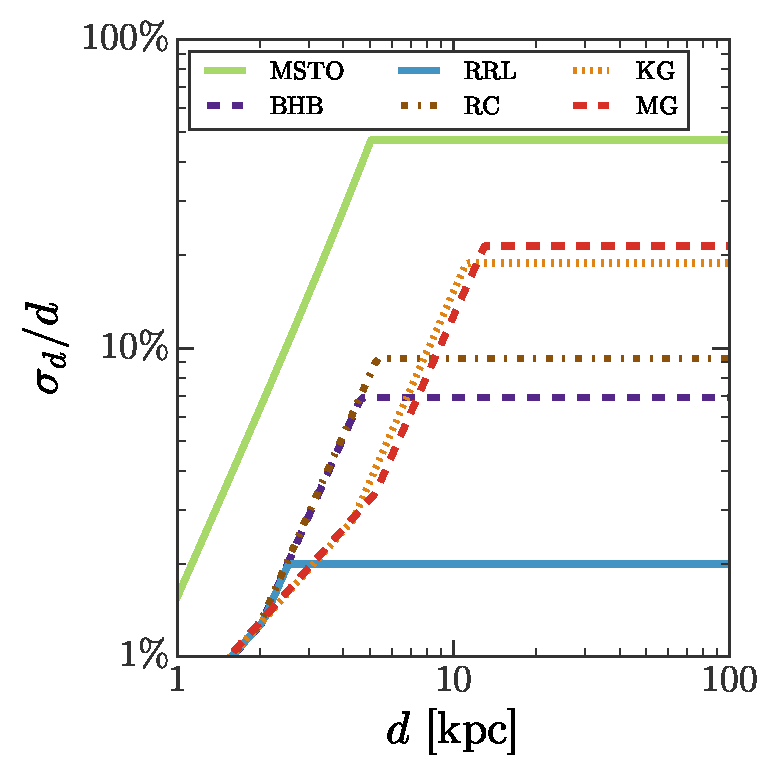
\includegraphics[width=0.48\textwidth]{figures/ch0/frac-plx-err.pdf}
    }
    \subfloat{
      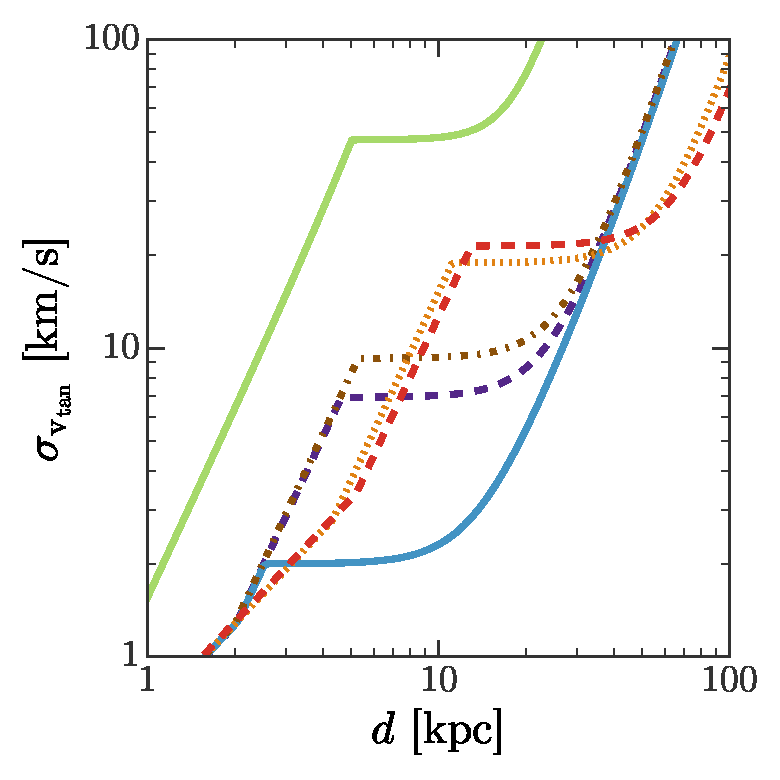
\includegraphics[width=0.48\textwidth]{figures/ch0/vtan-err.pdf}
    }
\caption{\todo{write this shite}}
\label{fig:gaiastellarpops}
\end{figure}

The \gaia\ mission is currently measuring parallaxes, proper motions, and radial
velocities for $\approx$$10^{8}$ stars in the Milky Way. The end-of-mission data
release from \gaia\ (expected in 2022) will provide astrometric measurements for
$\approx$$10^{9}$ stars. At distances $\gtrsim$10 kpc in the \mwhalo, the radial
velocity and parallax uncertainties will be large for all stellar types, but the
proper motion uncertainties will still be useful.
Figure~\ref{fig:gaiastellarpops} shows a summary of the expected distance and
tangential velocity uncertainties for each of the stellar tracers reviewed in
the previous section. Of particular note are the RR Lyrae stars, which will have
precise distance measurements and tangential velocity uncertainties
$\lesssim$$10~\kms$ out to 25 kpc.

Another highly anticipated survey for Milky Way \mwhalo\ science is the Large
Synoptic Survey Telescope \citep[LSST;][]{lsstsciencebook}. The telescope design
and large mirror of the LSST will enable deep imaging over a huge field of view
(magnitude limits of $\approx$24.5 for single-epoch images, $\approx$27.5 for
coadded images). The LSST will image most of the visible sky in five filters
every few nights, which will allow identification of faint time-variable stars
like RR Lyrae stars at extreme distances (out to $\approx$2--3 times the virial
radius of the Milky Way). At the faint end, the LSST will supercede the \gaia\
astrometry and provide proper motions better than $\lesssim$$1~{\rm mas}~{\rm
yr}^{-1}$ for stars with $r$-band magnitudes $20 \lesssim r \lesssim 24$. The
survey will begin science operations in 2022 with the first data release
expected about a year later.

Much of the \mwhalo\ will be mapped in sky position, distance, and proper motion
by the combination of \gaia\ and LSST; the last kinematic quantities needed are
radial velocities. Unlike multi-object spectroscopy---needed to obtain large
samples of radial velocities---imaging surveys do not scale in complexity with
the number of sources. Robotic fiber-positioning spectrographs
\citep{saunders12} have and will make it possible to simultaneously observe
1000s of stars, but are expensive to maintain and don't scale much above this
number. Combined with the longer exposure times needed to obtain high signal-to-
noise spectra, obtaining spectroscopy for a volume of stars comparable to the
astrometric sources in \gaia\ will be an enormous technological challenge.
However, it will be necessary in order to fully map out the chemical-abundance
structure of and measure radial velocities for these sources. Many ongoing
efforts \citep[e.g.,][]{rave06, segue08, apogee15, galah15} have obtained
spectra of varied resolution for $\approx$1 million stars around the Galaxy. The
future Dark Energy Spectroscopic Instrument \citep[DESI;][]{desi-whitepaper}
will take spectra of an additional $\approx$$10^7$ stars, but this is still
orders of magnitude below the number needed to have complete 6D phase-space
coverage for the entire Milky Way halo.

% [...maybe add something about focusing on particular tracer?]

\section{Outline of thesis}

Rich kinematic data impending, what can we learn about the dark matter halo of the Milky Way?

\todo{stuff}
